\subsection{ソフトウェア設計の記録}

設計プロセスの成果は、設計者の頭の中だけに残しておくべきではない。設計記録は、問題、解決策、判断、根拠を関係者へ伝えるためのものである。設計記録には、文章、図、表、モデル、プロトタイプ、コード片などが含まれる。

設計記録の目的は、実装者に作るべきものを示すことだけではない。顧客、テスト担当、品質保証担当、認証担当、保守担当も設計情報を必要とする。したがって、どの設計情報を、誰に向けて、どの詳細度で記録するかを意識して決める必要がある。

\begin{pointbox}{基本方針}
設計記録は「すべてを詳細に書く」ことが目的ではない。読者、利用目的、リスク、保守期間に応じて、必要な設計知識を取り出しやすい形で残すことが目的である。
\end{pointbox}

\subsubsection{モデルに基づく設計}

\term{モデルに基づく設計}{Model-Based Design, MBD} は、モデルを設計記録の中心に置く方法である。従来の文書中心の設計では、自然言語と非形式的な図を使うため、曖昧さや不完全さが残りやすい。また、必要な情報が複数文書に分散し、理解や分析が難しくなる。

モデルに基づく設計では、ツールが設計情報を整理し、表示し、分析できる。たとえば、モデルの一部をアニメーションやシミュレーションで確認したり、仮定を変えた場合の影響を調べたり、要求から設計、設計からテストへの追跡を支援したりできる。

\term{モデル駆動開発}{Model-Driven Development, MDD} は、モデルを開発プロセスの主要成果物として使い、コード生成や検証へつなげる考え方である。

\par\smallskip
\begin{center}
\centering
\IfFileExists{assets/generated_figures/ch03/fig-ch03-07.png}{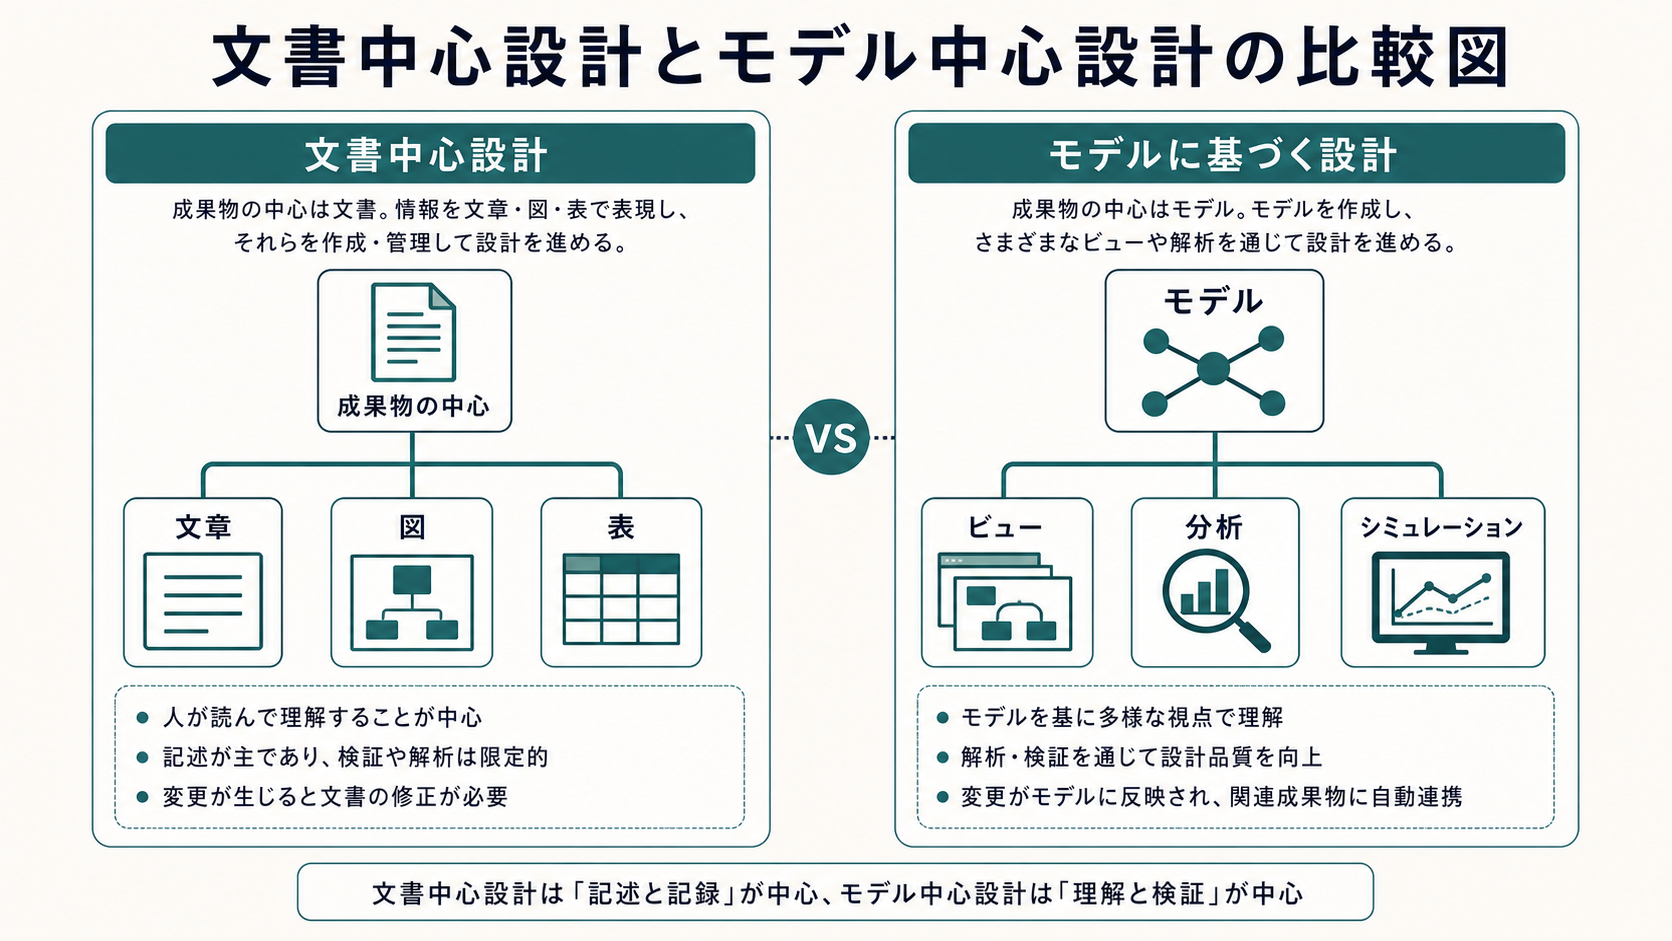
\includegraphics[width=0.96\linewidth]{assets/generated_figures/ch03/fig-ch03-07.png}}{\fbox{\parbox[c][48mm][c]{0.9\linewidth}{\centering 画像生成待ち\\文書中心設計とモデル中心設計の比較図}}}
\par\smallskip
\refstepcounter{figure}\label{fig:ch03-07}図 \thefigure: 文書中心設計とモデル中心設計の比較図
\end{center}
図 \thefigure は、文書中心設計とモデル中心設計の比較図を視覚的に整理したものである。
\par\smallskip

\subsubsection{構造設計記述}

\term{構造設計記述}{Structural Design Description} は、ソフトウェアの静的な構造を表す。つまり、どの構成要素があり、それらがどう関係し、どの責務を持つかを示す。

代表的な記法は次のとおりである。

\par\smallskip\noindent\refstepcounter{table}\label{tab:ch03-04}表 \thetable: 構造設計記述の整理\par\smallskip
表 \thetable は、構造設計記述の整理を比較・確認しやすい形で整理したものである。\par\smallskip
\begin{longtable}{L{42mm}L{112mm}}
\toprule
記法 & 説明 \\
\midrule
\endhead
クラス図・オブジェクト図 & クラス、オブジェクト、属性、操作、関連を表す。オブジェクト指向設計でよく使われる。 \\
コンポーネント図 & 交換可能な構成要素と、その提供・要求インタフェースを表す。 \\
CRCカード & クラス名、責務、協調相手をカード形式で整理する。初期設計や会話に向く。 \\
配置図 & ソフトウェアをどの物理ノードや実行環境へ配置するかを表す。 \\
実体関連図 & データの実体、属性、関係を表す。データ設計でよく使われる。 \\
インタフェース記述言語 & 構成要素が公開する操作名、型、引数、戻り値などを記述する。 \\
構造チャート & プログラムの呼び出し構造を表す。どのモジュールがどのモジュールを呼ぶかを示す。 \\
\bottomrule
\end{longtable}

\subsubsection{振る舞い設計記述}

\term{振る舞い設計記述}{Behavioral Design Description} は、ソフトウェアが時間の中でどのように動くかを表す。処理の流れ、イベントへの反応、状態変化、入力と出力の関係などを示す。

代表的な記法は次のとおりである。

\par\smallskip\noindent\refstepcounter{table}\label{tab:ch03-05}表 \thetable: 振る舞い設計記述の整理\par\smallskip
表 \thetable は、振る舞い設計記述の整理を比較・確認しやすい形で整理したものである。\par\smallskip
\begin{longtable}{L{42mm}L{112mm}}
\toprule
記法 & 説明 \\
\midrule
\endhead
活動図 & 処理の流れ、分岐、並行活動、入力、出力を表す。 \\
相互作用図 & オブジェクトや構成要素間のメッセージ交換を表す。通信図とシーケンス図が代表である。 \\
データフロー図 & 処理要素間を流れるデータを表す。セキュリティ分析にも使える。 \\
決定表・決定図 & 条件の組合せと、それに対応する動作を表す。複雑な業務規則に向く。 \\
フローチャート & 制御の流れと処理順序を表す。 \\
状態遷移図・状態チャート & 状態、イベント、遷移、状態ごとの振る舞いを表す。 \\
形式仕様言語 & 数学的な記法で、インタフェースや振る舞いを厳密に定義する。 \\
擬似コード・プログラム設計言語 & プログラムに近い形で処理手順を表す。詳細設計やアルゴリズム説明に使う。 \\
\bottomrule
\end{longtable}

\par\smallskip
\begin{center}
\centering
\IfFileExists{assets/generated_figures/ch03/fig-ch03-08.png}{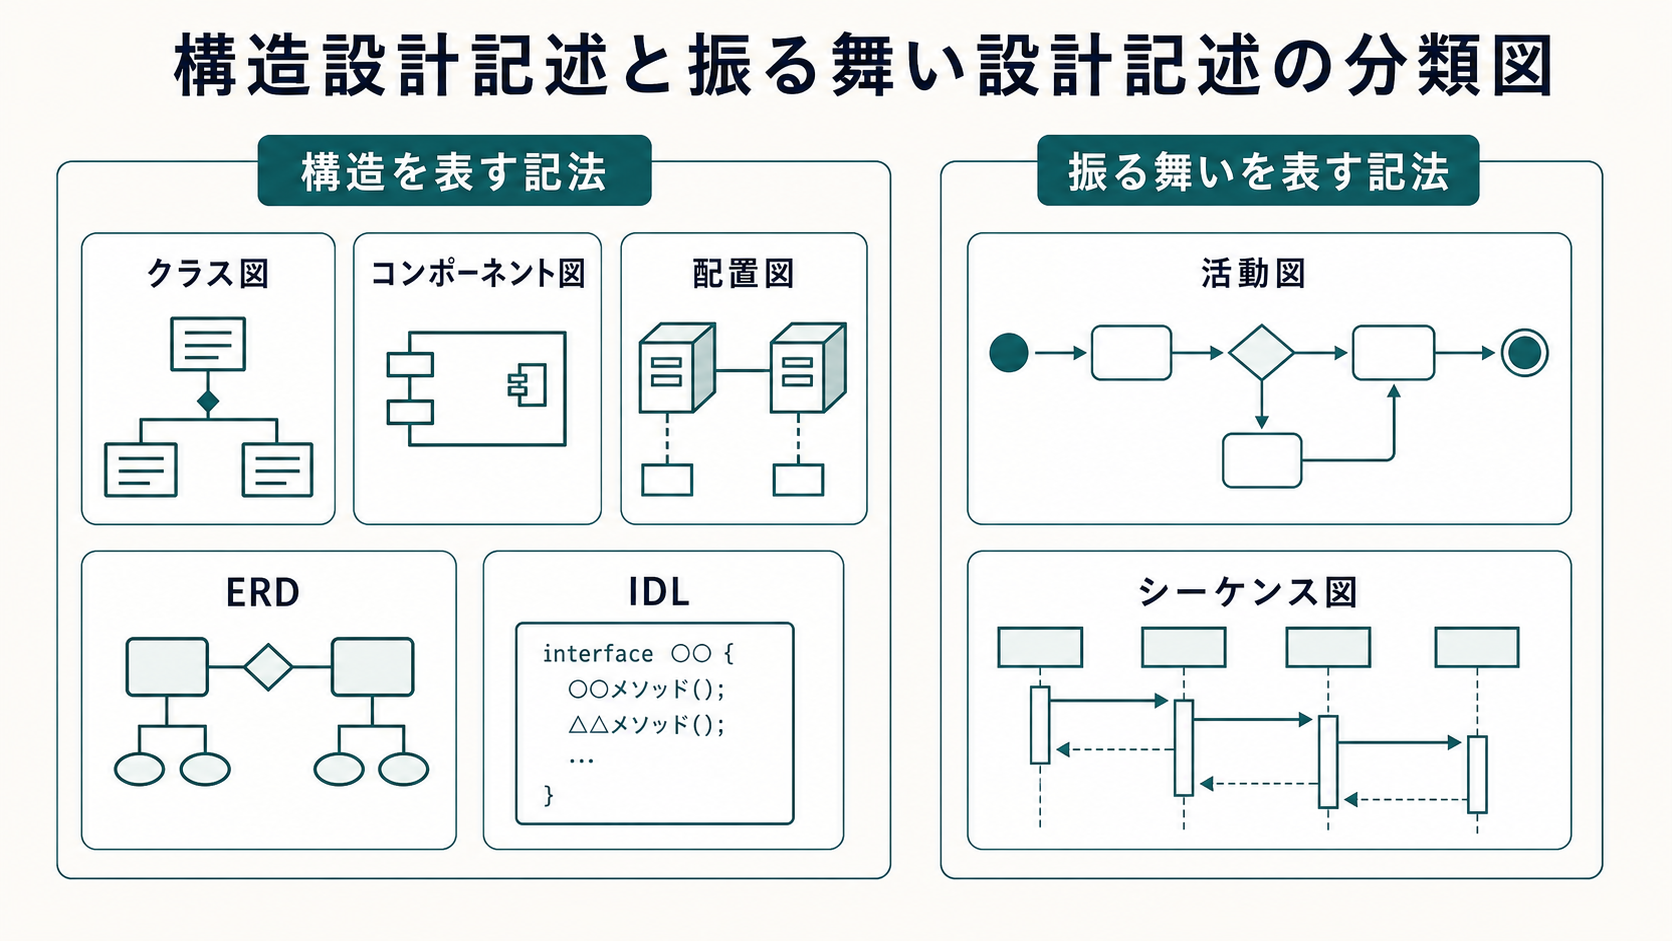
\includegraphics[width=0.96\linewidth]{assets/generated_figures/ch03/fig-ch03-08.png}}{\fbox{\parbox[c][48mm][c]{0.9\linewidth}{\centering 画像生成待ち\\構造設計記述と振る舞い設計記述の分類図}}}
\par\smallskip
\refstepcounter{figure}\label{fig:ch03-08}図 \thefigure: 構造設計記述と振る舞い設計記述の分類図
\end{center}
図 \thefigure は、構造設計記述と振る舞い設計記述の分類図を視覚的に整理したものである。
\par\smallskip

\subsubsection{設計パターンとスタイル}

\term{設計パターン}{Design Pattern} は、特定の文脈で繰り返し現れる問題に対する一般的な解決策である。設計パターンは、過去に有効だった設計上の慣用句を共有するための語彙である。

代表的な分類は、生成、構造、振る舞いである。
\begin{itemize}
  \item \term{生成パターン}{Creational Pattern}：オブジェクトや部品の生成方法を扱う。ビルダー、ファクトリ、プロトタイプ、シングルトンなどがある。
  \item \term{構造パターン}{Structural Pattern}：部品の組み合わせ方を扱う。アダプタ、ブリッジ、コンポジット、デコレータ、ファサード、プロキシなどがある。
  \item \term{振る舞いパターン}{Behavioral Pattern}：責務の分担や相互作用を扱う。コマンド、イテレータ、メディエータ、オブザーバ、状態、戦略、テンプレート、ビジタなどがある。
\end{itemize}

\term{スタイル}{Style} は、より大きな構造の特徴を表す場合に使われることが多い。たとえば、階層化、パイプ・アンド・フィルタ、クライアントサーバ、イベント駆動などは、システム全体または大きな部分の設計方針として現れる。

\par\smallskip
\begin{center}
\centering
\IfFileExists{assets/generated_figures/ch03/fig-ch03-09.png}{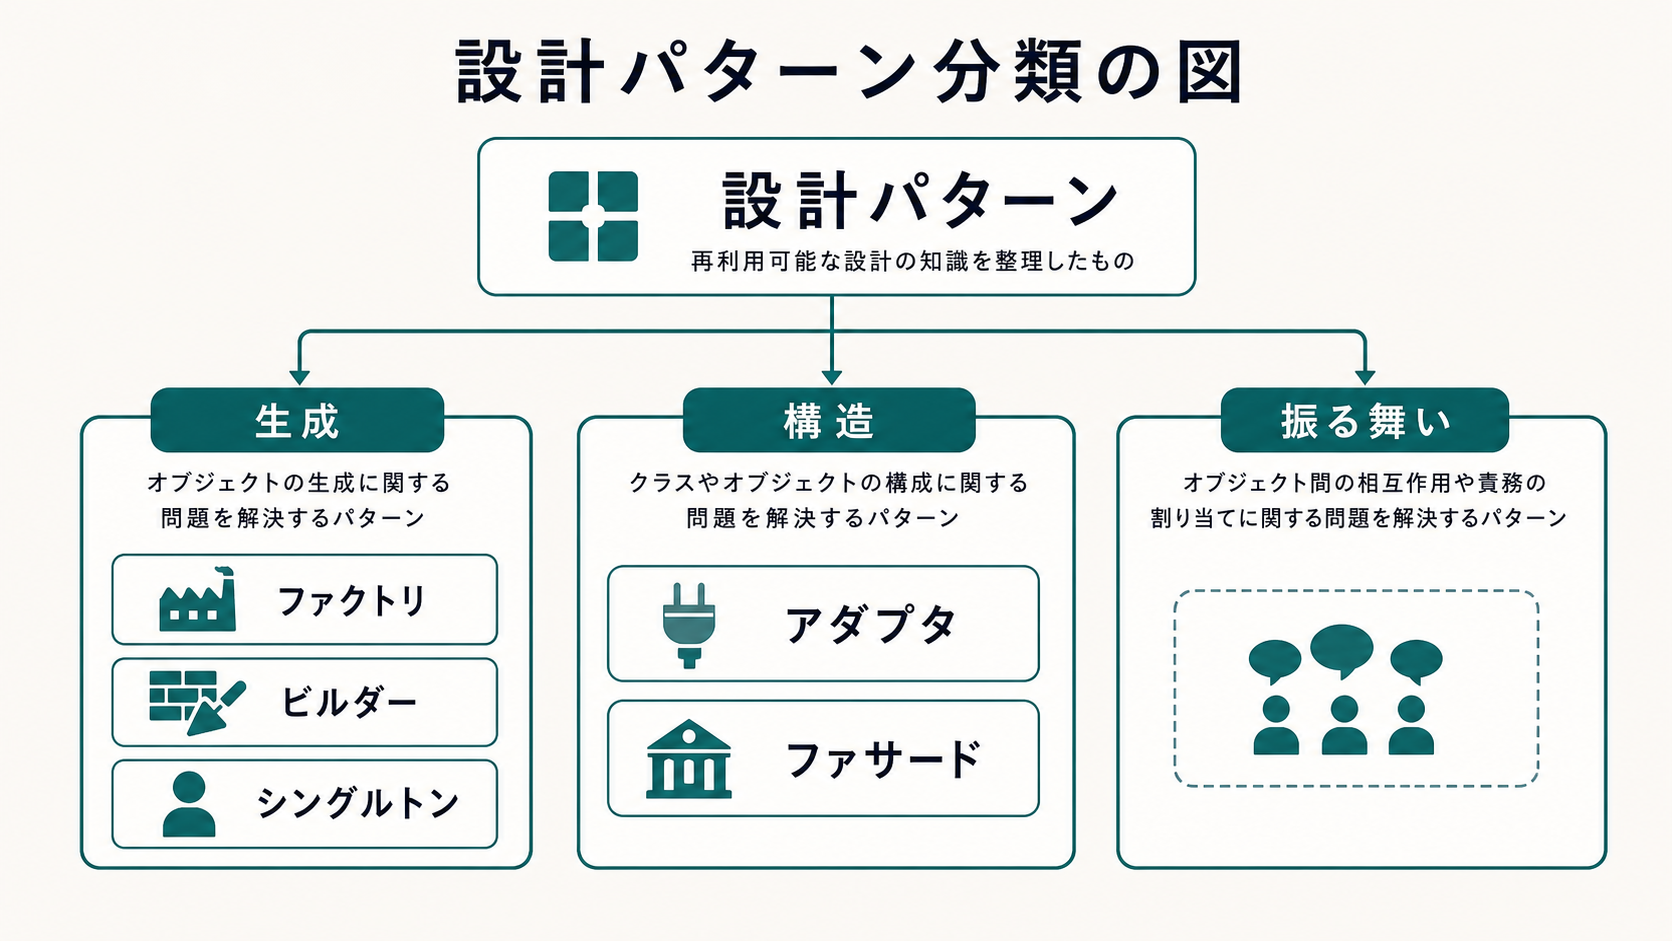
\includegraphics[width=0.96\linewidth]{assets/generated_figures/ch03/fig-ch03-09.png}}{\fbox{\parbox[c][48mm][c]{0.9\linewidth}{\centering 画像生成待ち\\設計パターン分類の図}}}
\par\smallskip
\refstepcounter{figure}\label{fig:ch03-09}図 \thefigure: 設計パターン分類の図
\end{center}
図 \thefigure は、設計パターン分類の図を視覚的に整理したものである。
\par\smallskip

\subsubsection{専用言語と領域固有言語}

設計表現は、構造と振る舞いの二分法だけで整理できるとは限らない。たとえば、利用者インタフェース設計では、画面の構造、操作の流れ、入力制約、表示規則が混ざる。また、安全性や信頼性の領域では、その分野に特化した記法が発達している。

\term{領域固有言語}{Domain-Specific Language, DSL} は、特定の業務領域や技術領域の概念を直接表すための言語である。汎用プログラミング言語ではなく、その領域の語彙を使って設計や実装に近い表現を行う。例として、シミュレーション、リアルタイムシステム、ゲーム開発、利用者インタフェース、テスト開発、言語処理などの領域向けDSLがある。

DSLの利点は、領域の専門家が理解しやすい語彙で表現できることである。一方、DSLを作るには、言語仕様、構文解析、生成、保守の負担がある。したがって、繰り返し使う価値がある領域で特に有効である。

\subsubsection{設計根拠}

設計根拠 は、なぜその設計判断をしたかを説明する情報である。設計根拠には、前提、検討した代替案、採用基準、トレードオフ、却下した案の理由が含まれる。

設計チームにとって、現在の判断理由は明らかに見えることが多い。しかし、数か月後、数年後、または担当者交代後には、その理由が失われる。設計根拠を記録すれば、保守担当者は「なぜこの構造なのか」「なぜ別案を採らなかったのか」を理解しやすい。

却下した判断を記録することも有用である。前提や制約が変わったとき、以前は却下された案が有効になる場合がある。逆に、過去に明確な理由で却下された案を、理由を忘れて再び採用してしまうことを防げる。

\begin{pointbox}{実務の見方}
設計根拠は、巨大な説明文である必要はない。「判断」「理由」「代替案」「影響」「未解決事項」を短く残すだけでも、後の保守で大きな価値を持つ。
\end{pointbox}
